\section{Implementation and tests}

\todo{The COACHES robots are under construction, so we use a simulator...}


\begin{figure}
\centering
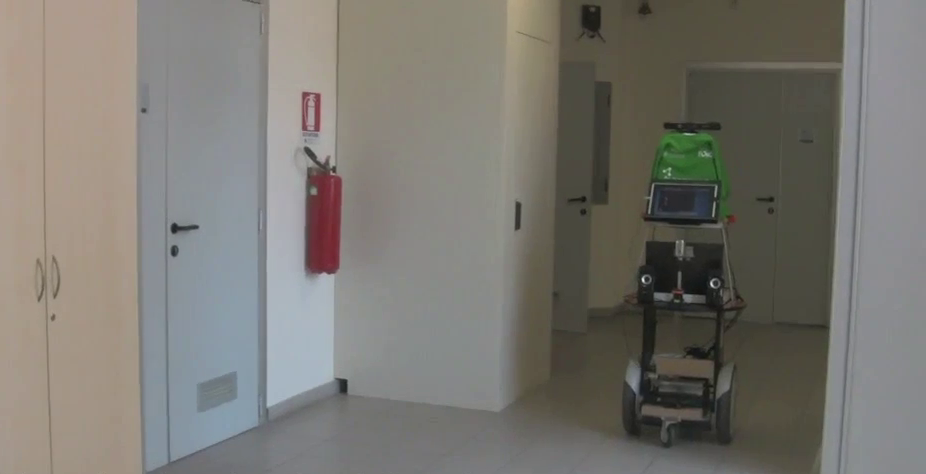
\includegraphics[width=0.75\textwidth]{fig/diago.png}
\caption{Diago robot at Sapienza University.}
\label{fig:diago}
\end{figure}



\subsection{Simulator environment}

The simulation environment is based on 2D Stage simulator, which is integrated in the ROS infrastructure. The choice of a 2D simulator (instead of a 3D one) is motivated by: 1) the need of modeling and testing high-level behaviors of the robot that does not involve 3D perception, 2) the possibility of using the simulator for multiple robots and other moving elements representing people in the environment, 3) the possibility of using the simulator on standard laptop, thus not requiring advanced graphical cards for running 3D simulations.

\begin{figure}
\centering
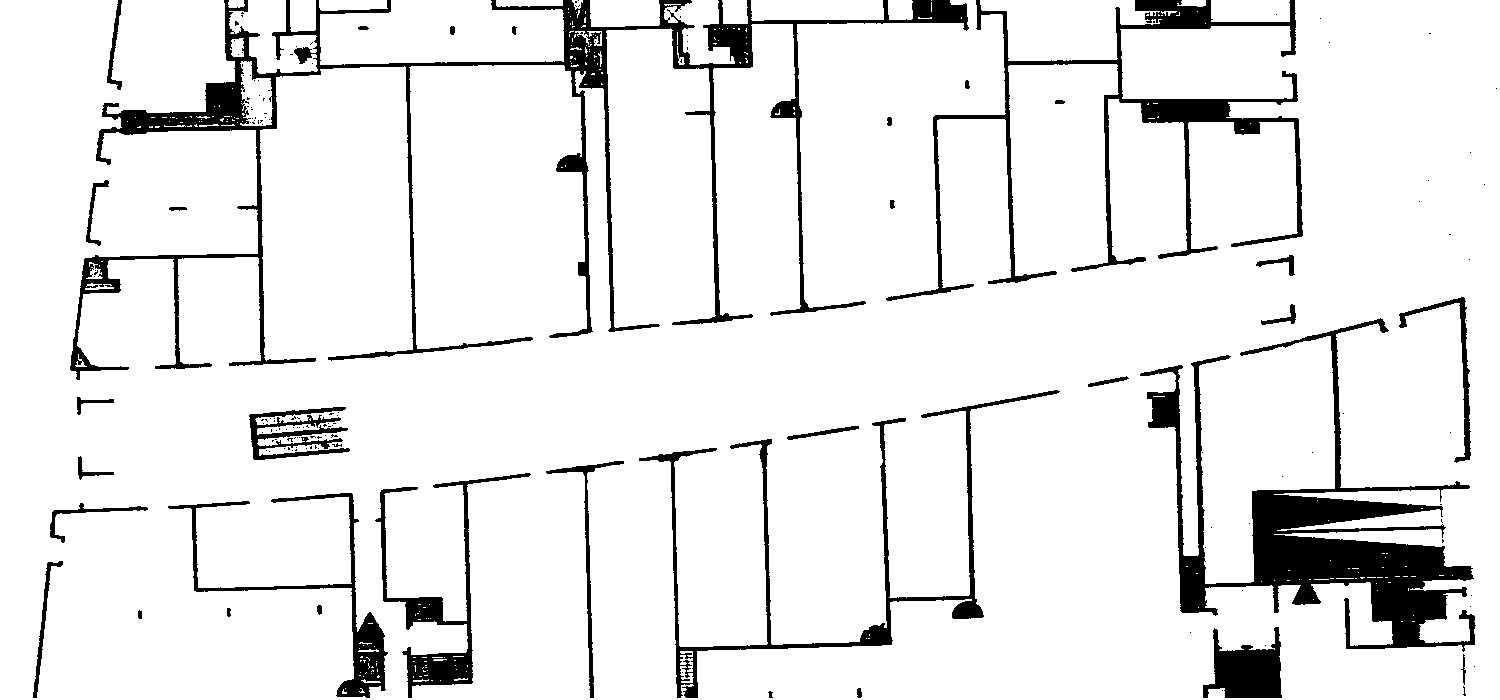
\includegraphics[width=0.95\textwidth]{fig/Rive1.png}
\caption{2D map of the \emph{Rive de l'orne} shopping center.}
\label{fig:stage}
\end{figure}


In the Stage simulator the following map of the \emph{Rive de l'orne} shopping center has been realized. In Figure \ref{fig:stage} a section of the shopping mall in which we will deploy the prototypes is shown.
Additional maps have been realized for reproducing the environments of the partners in which some experiments will be performed.

The Stage environment models one or more robots that have the same 2D sensor and actuator configurations of the real ones and some additional mobile obstacles that represent people moving in the environment. Several behaviors can be tested in this simulated environment such as: 2D perception of human behaviors, human-robot social navigation (e.g., following a person or guiding a person), safe navigation in the environment.

The Stage environment has been fully realized and tested and this configuration will be used as a reference also for the development of the real robotic system.

\subsection{Plan generation and execution tests}

The following tests have been performed in the simulator to verify the suitability of the proposed software architecture and of its components. In particular, we have used the simulated environment to assess the suitability of the AI components described in the previous section.

\todo{Describe some runs in simulation}
